\chapter{Simultaneous Depth and Pose from Light Fields}

In Chapter 3, we saw that previous work has produced a variety of approaches to depth estimation and visual odometry, using both data-driven and hand crafted solutions. In this chapter, we propose a novel pipeline that behaves similarly to the pipelines described in Chapter 3, with the key distinction of operating on 4D, as opposed to 2D data. The contributions of previous work focus on the use of monocular and stereo image data, while this chapter focuses on developing a pipeline that employs the full breadth of geometric information in the light field. The first section of this chapter describes the tools and methodologies of acquiring a suitable dataset, while the second part derives the pipeline used for our experiments.

\section{Data Acquisition}

\subsection{Ground Truth Pose Data}

\begin{figure}[h]
    \centering 
    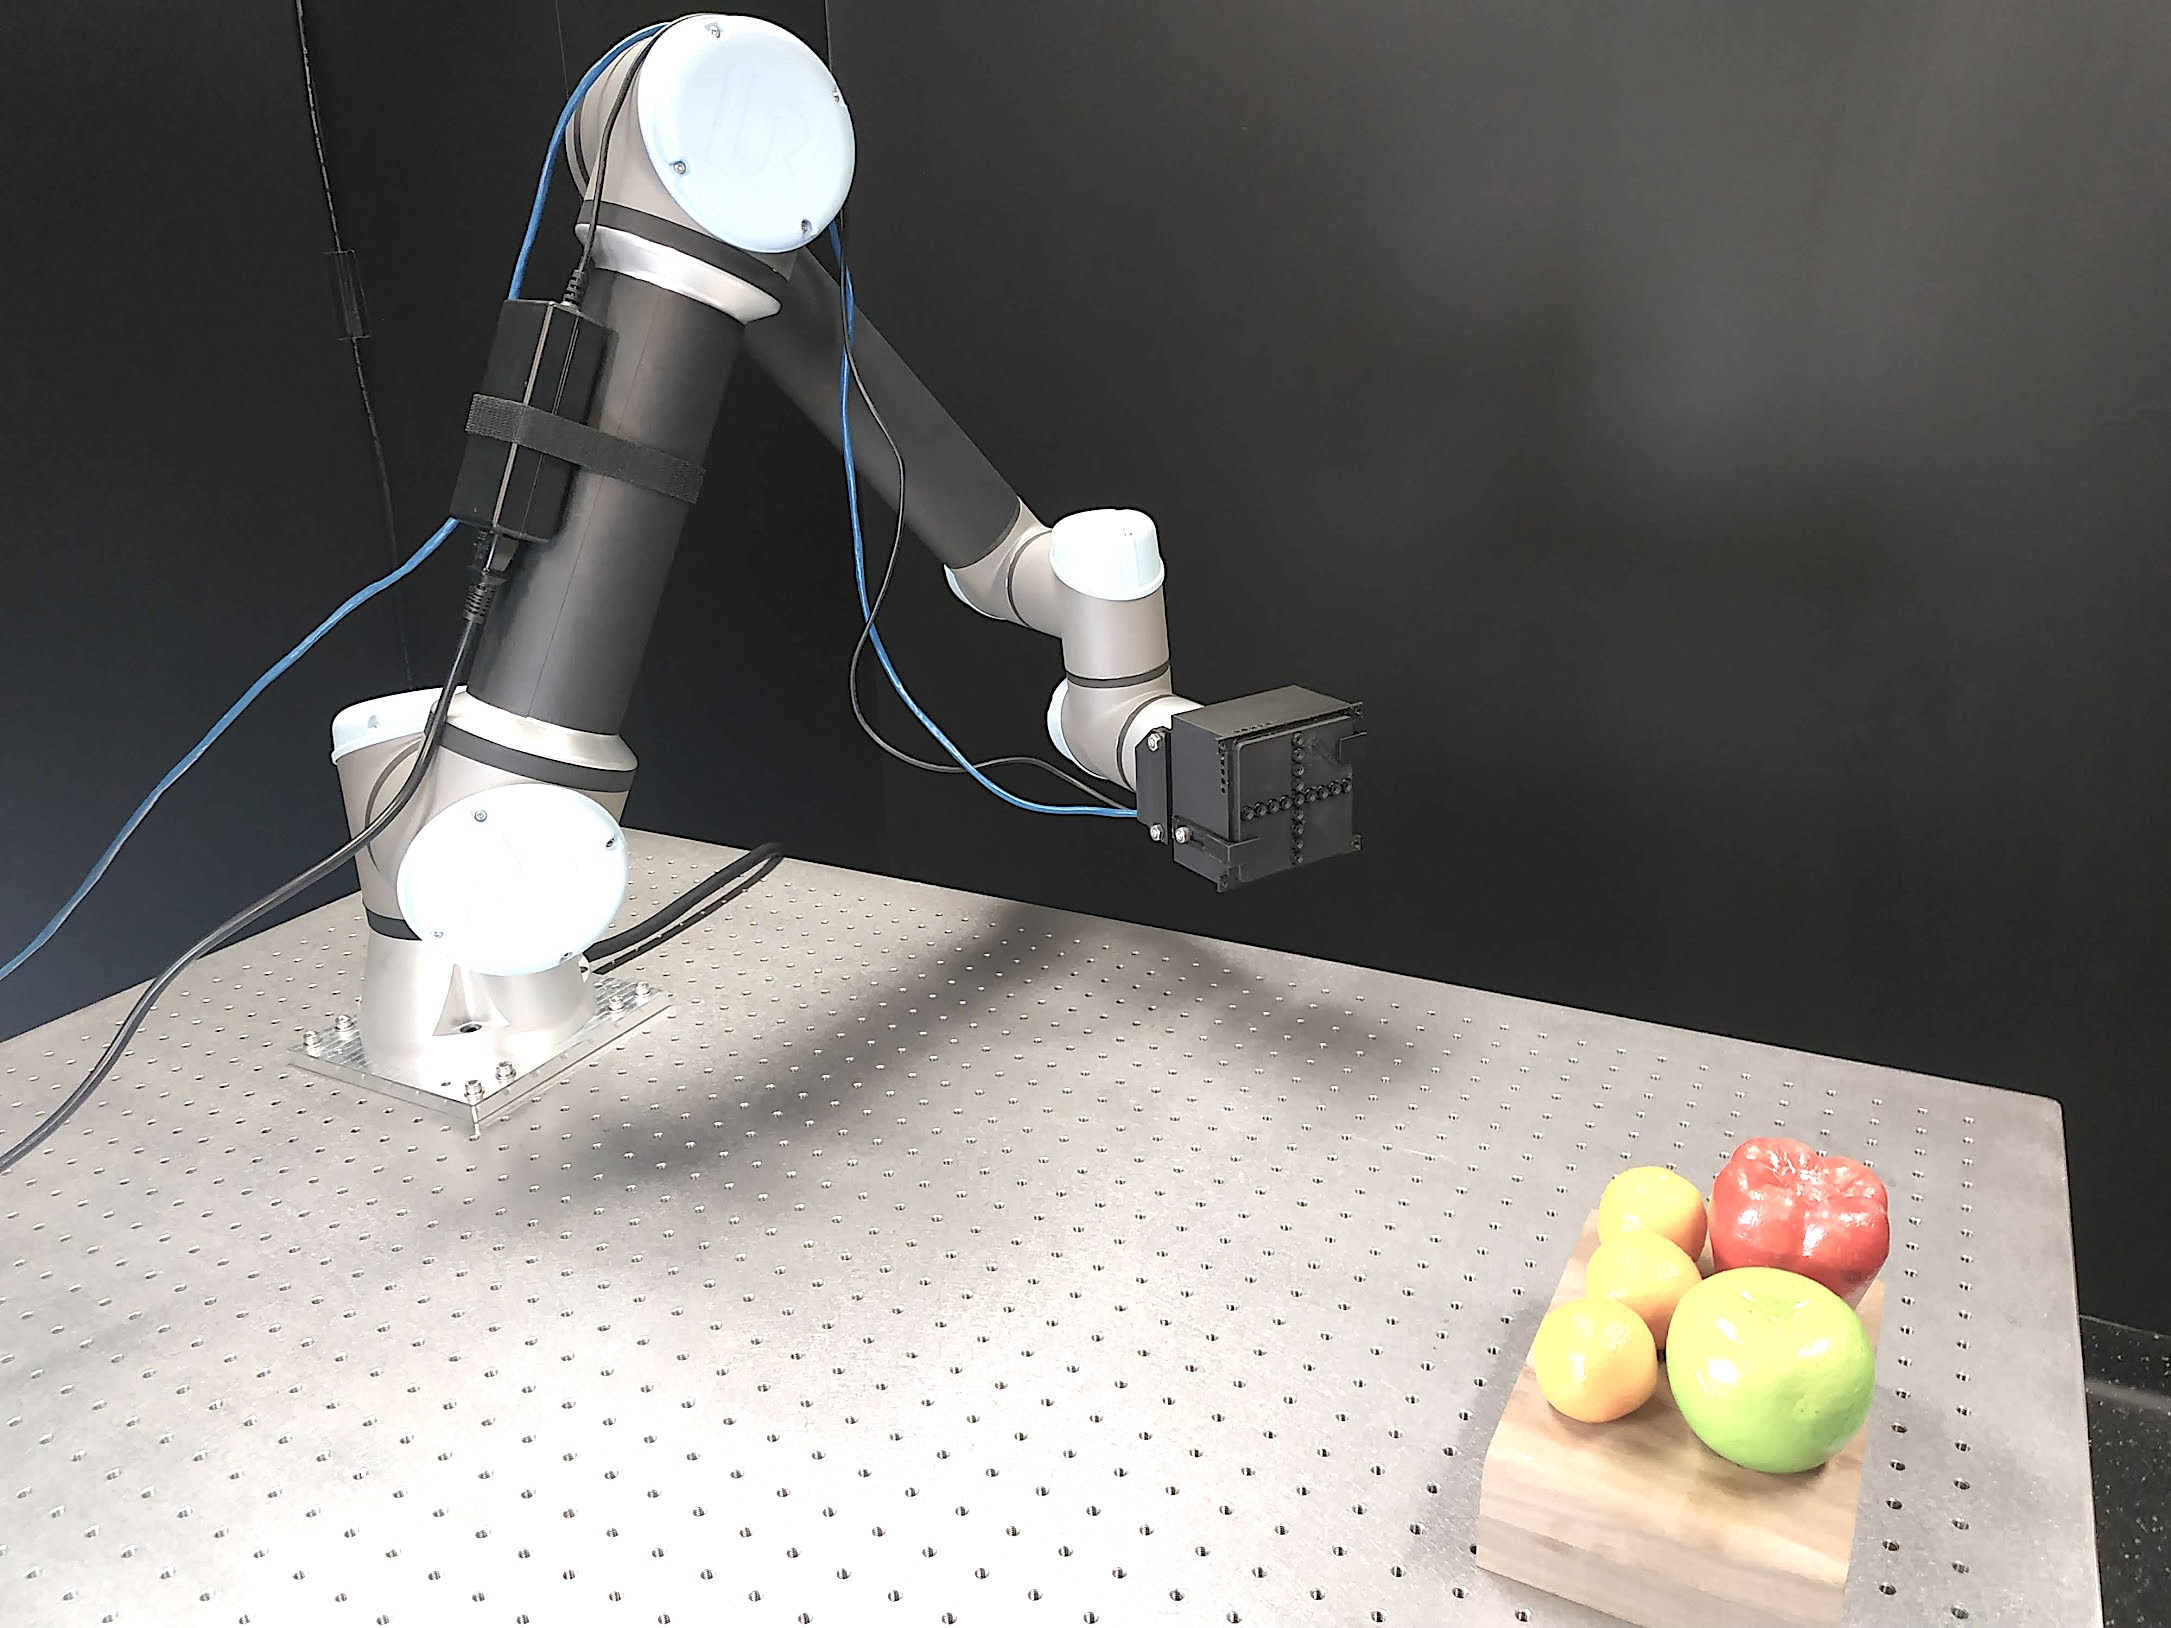
\includegraphics[width=4.5in]{images/experimentalsetup2.jpg}
    \caption{The experimental setup utilises a Universal Robots UR5E robotic arm to precisely measure ground-truth pose to allow effective evaluation of the projects visual odometry results.}
\end{figure}

Important to this work is a strong evaluation framework. Existing datasets such as KITTI and CityScapes benefit from state-of-the-art sensor suites including inertial sensors and lidar, allowing researchers to effectively benchmark their results. Similarly, this thesis places a strong emphasis on validation using ground truth data. One of the primary tasks for evaluation is visual odometry, and so ground-truth pose data for each image is a valuable resource. In this project, pose is collected by attaching the camera to a Universal Robots UR5E robotic manipulator, which is capable of sensing to a high degree of accuracy the pose of the end effector. Furthermore, the UR5E is able to perform accurate movements and trajectories with payloads of up to 5 kilograms, making it a suitable robotic mount for the camera. 

\subsubsection{Manipulator-Camera Interface Adapter}
The UR5E uses a standard interface plate for attaching end-effectors such as gripping tools. The camera on the other hand, despite its excellent construction, is an early prototype provided by EPIImaging, without a physical adapter interface for the UR5E manipulator. We therefore fabricate our own mount for the device, taking into consideration the camera's ventilation and cabling requirements. A two-piece adapter was designed in SolidWorks and fabricated using a fused deposition modelling (FDM) platform with polylactic acid (PLA) filament. 

\subsubsection{Manipulator Control}
A client library for communicating with the UR5E was developed in python, establishing a TCP/IP connection with the robot over the local network, allowing both movement commands to be sent to the robot, and feedback data about the end-effector's pose to be streamed back to the client PC. The client library also provides functionality for computing trajectories and corresponding joint angles, using the PyBullet \cite{pybullet2017} physics engine and the known kinematic model. One useful trajectory function from our library procedurally generates waypoints while keeping the camera's field-of-view trained on the scene, using a stringent collision-checking mechanism to enable autonomous data-capture. 

\subsection{Imagery}
The specific imaging device being used is manufactured by EPIImaging, and consists of 17 subapertures. The communication interface with the camera is a network connection serving image data using the HTTP protocol via a REST API. Both rectified and un-rectified imagery can be retrieved, and the format of the returned data is a $17\times 3 \times 1280 \times 960$ stream of raw bytes representing 8-bit pixel values from each of the 17 sensors. A simple client library was developed in python to automate API requests, and perform decoding of the pixel data.

\newpage

\section{Depth and Visual Odometry Pipelines}
In this section, we derive a pipeline for simultaneous depth and visual odometry using light field data. Our pipeline is constructed modularly, so to build a precise intuition for how our pipeline operates, we begin by describing the functions of each individual module. We first introduce the CNN modules used to estimate pose and depth. Subsequently we'll discuss strategies for forming meaningful loss-functions to train our pair of networks using a photometric-warp loss-module. Next, we launch a discussion on the input formats, altering how light field data is fed to our networks, discussing the comparable advantages and disadvantages of each. Finally, we introduce some modifications to the photometric-warp loss-module that sacrifices some flexibility in exchange for more robust depth and pose estimates that more-fully exploit information in the light field. 

\subsection{Pose Estimation}

We treat pose estimation as a regression problem, estimating three translational components [X, Y, Z] and three rotational components [Rx, Ry, Rz]. We perform this regressions with a convolutional network, which we call `PoseNet', in line with previous works. This network architecture is fully convolutional, meaning that in principle it produces the correct number of outputs for any 2D input.

\begin{table}[h]

    \caption{PoseNet Convolutional Network Architecture}
    \centering
    \begin{tabular}{@{}llllll@{}}
        \toprule
        Layer               & Kernel Size   & Output Channels   & Stride    & Padding   & Activation\\ 
        \midrule
        Conv1               & 7             & 16                & 2         & 3         & ReLU      \\ 
        Conv2               & 5             & 32                & 2         & 2         & ReLU      \\ 
        Conv3               & 3             & 64                & 2         & 1         & ReLU      \\ 
        Conv4               & 3             & 128               & 2         & 1         & ReLU      \\
        Conv5               & 3             & 256               & 2         & 1         & ReLU      \\
        Conv6               & 3             & 256               & 2         & 1         & ReLU      \\
        Conv7               & 3             & 256               & 2         & 1         & ReLU      \\
        Output              & 1             & 1                 & 1         & 1         & -         \\ 
        \bottomrule
    \end{tabular}
    \label{posenet-layers}
\end{table}

Importantly, the translation and rotation are regressed relative to the \textit{camera} coordinate frame of the first image, whereas the UR5E returns absolute position and orientation in the \textit{world} coordinate frame. To validate our predictions we therefore need to compute the relative translation $P_{t1 \rightarrow t2}$ and rotation $R_{t1 \rightarrow t2}$ of the two images, given their absolute positions $P_{t1}, P_{t2}$ and orientation $R_{t1}, R_{t2}$ in the world frame. Concatenating translation and rotation into a single transform matrix $T = [R|t]$ allows us compute both relative rotation and translation in a single step, as:

\begin{equation}
T_{t1 \rightarrow 2} = T_{t1}^{-1} T_{t2}.
\end{equation}

Intuitively, this computation first computes the transform from pose 1 to the world frame, then from the world frame to pose 2. We can decompose this matrix into 3 translational and 3 rotational components. 


\subsection{Depth Estimation}

Depth estimation is similarly modeled as a regression problem, with the same number of outputs as inputs. The depth estimation module uses the fully-convolutional encoder-decoder `DispNet' architecture \cite{mayer2015dispnet}. Skip connections from the encoder to the decoder mean the decoding layers are able to access both high level features and low level features on either side of the latent space. Prior work \cite{zhou2017unsupervised} has demonstrated that predicting depth maps at multiple scales improves photometric reconstruction error by enforcing some level of local smoothness. In practice, this helps the network learn to predict depth in challenging, textureless regions of the image. 

\begin{table}[h]

    % \caption{DispNet Convolutional Network Architecture}
    \centering
    \caption{DispNet Convolutional Network Architecture.}
    \begin{tabular}{@{}l|lllllll@{}}

        \toprule
        & Layer       & Kernel Size   & Concatenate   & Output Channels   & Stride    & Padding   & Activation\\ \midrule
        \multirow{7}{*}{\rotatebox{90}{Encoder}}    
        &Conv1       & 7             & -             & 32                & 2         & 3         & ReLU     \\ 
        &Conv2       & 5             & -             & 64                & 2         & 2         & ReLU      \\ 
        &Conv3       & 3             & -             & 128               & 2         & 1         & ReLU      \\ 
        &Conv4       & 3             & -             & 256               & 2         & 1         & ReLU      \\
        &Conv5       & 3             & -             & 512               & 2         & 1         & ReLU      \\
        &Conv6       & 3             & -             & 512               & 2         & 1         & ReLU      \\
        &Conv7       & 3             & -             & 512               & 2         & 1         & ReLU      \\ \midrule
        \multirow{9}{*}{\rotatebox{90}{Decoder}} 
        &UpConv7     & 3             & Conv6         & 512               & 2         & 1         & ReLU      \\
        &UpConv6     & 3             & Conv5         & 512               & 2         & 1         & ReLU      \\
        &UpConv5     & 3             & Conv4         & 256               & 2         & 1         & ReLU      \\
        &UpConv4     & 3             & Conv3         & 128               & 2         & 1         & ReLU      \\
        &UpConv3     & 3             & Conv2         & 64                & 2         & 1         & ReLU      \\
        &UpConv2     & 3             & Conv1         & 32                & 2         & 1         & ReLU      \\
        &Output2     & 3             & -             & 1                 & 1         & 1         & Sigmoid   \\
        &UpConv1     & 3             & -             & 32                & 2         & 1         & ReLU      \\
        &Output1     & 3             & -             & 1                 & 1         & 1         & Sigmoid   \\
        \bottomrule
    \end{tabular}
    
    \vspace{4mm}{}
    \textit{Layers prefixed with `Conv' or `Output' are convolutional layers, and those prefixed with `UpConv' use the transposed-2D-convolution to upsample the preceeding layer.}
    
    \label{dispnet-layers}
\end{table}


\subsection{Photometric Warp Loss}
We have now described one CNN tasked with estimating a per-pixel depth map of the scene, and another which estimates the 6-degree-of-freedom pose between two frames of video. The challenge is now to provide a supervision signal that sufficiently constrains these networks to actually perform the tasks of depth and pose estimation. 

\subsubsection{A Differentiable Loss Function with Image Based Rendering}

As described in Chapter 3, given an estimate for these two pieces of information, we are able to synthesise approximate images of the scene as seen from a nearby viewpoint. We take advantage of this fact to form a photometric-warp loss, similar to \cite{zhou2017unsupervised}. 

As described in Chapter 3, the procedure for this is to first project each pixel from the first light field $LF_1$ to a 3D point cloud using the known camera intrinsics and estimated depth values. If we have regressed a depth map $D(s_0, t_0, u, v)$ for the sub-aperture $s_0, t_0$, we can for each pixel $[u, v]^T$ project its position to a 3D point cloud $Q$. 

\begin{equation}
    Q = D(s_0, t_0, u, v) K^{-1}\begin{bmatrix}u \\ v \\ 1\end{bmatrix} \quad \forall u, v.
\end{equation}

The 3D coordinate $Q$ is then projected onto the sensor plane of $LF_2$, at the pixel coordinate $[s_0,t_0,\hat{u},\hat{v}]$. This relies on our estimate of the relative pose $[R|t]$ from the first to the second camera origin.

\begin{equation}
    [s_0, t_0, \hat{u}, \hat{v}] = K[R|t]Q \quad \forall Q
\end{equation}

The pixels $[s_0, t_0, \hat{u}, \hat{v}]$ are subsequently sampled to populate a new array, forming our synthesised image. This transform is equivalent to constructing a 3D model of the scene using our depth values, moving an imaginary camera by $[R|t]$ and taking a virtual snapshot of the scene from this new angle, the snapshot being the resulting photometric warp.

More broadly, the practice we have described here is referred to as `image based rendering', which is a related, but slightly different paradigm from the rasterization, shaders and textures typically used in graphics-based rendering engines. In image based rendering, we instead synthesise viewpoints using existing image data. In a sense, image based rendering simply shuffles the pixels of an existing image around, according to some pre-defined rules. In our case, we derive the shuffling-rules using 3D data inferred by our depth and pose networks. The perceptive reader may have noticed that the pixel value $p_2 = [s_0, t_0, \hat{u}, \hat{v}]$ is continuous in $u$ and $v$, while pixel coordinates should be discretely valued. A naive solution is to discretise the coordinate $p_2$ by sampling its nearest-neighbouring pixel. We must remember however that neural networks rely on the chain rule of calculus to perform back-propagation, and so whatever sampling regime we choose must be differentiable. We therefore turn to bilinear sampling, as described in Chapter 3 as a differentiable sampling mechanism. Its operation and derivatives are described in equations 3.3-3.5.


\subsection{Input Methods}

This work tackles an interesting and unique challenge, of how to feed sparse light field data to convolutional neural networks. We summarise this challenge as:

\textit{Given sparse 4 dimensional data, how best can we arrange that data as 2 dimensional slices in a valuable and informative way to a convolutional network for the purposes of visual odometry and depth estimation.}

As we have seen in Chapter 3, this problem has been approached in prior work, usually with the assumption that a complete 2D grid of 2D images is available. In this work however, the specific camera configuration prohibits arranging our data as a 2D grid of images without introducing significant redundant data. In a way, this forces us to consider more flexible and generalisable methods for processing light fields into constructive forms of 2 dimensional data. In this section, we suggest three experimental methods for ingesting light field data through neural networks. In the next chapter, we will present visual odometry and depth results using each of these methods.

\subsubsection{Volumetric Images}
The most straightforward of our three methods, this technique involves taking \textit{U, V} slices (perspective-projection images) of the light field, and stacking them along a 3rd axis (usually reserved for the colour-channels). The resulting image is an $H \times W \times N$ volume, where $H$ and $W$ are the height and width of the \textit{U, V} slice, and $N$ is the number of sub-apertures being sampled. This method is suggested, and tested by Wang et al. \cite{wang2016lfcnn} for material classification, who report improved results over conventional 2D imagery. Internally, we expect a convolutional network to learn features relating to parallax, occlusion and depth when exposed to data of this format.

\subsubsection{Focal Stacks}
Focal-stacks are constructed as a superposition of 2D images from several sub-apertures, creating interference in regions of the image that are `out-of-focus', while keeping `in-focus' elements of the image crisp. A focal stack specifically encodes depth in the form of interference at each region of the image. Thus, we might expect a CNN trained on this type of imagery to learn to decode in- and out-of-focus parts of the image, using this information to estimate depth and pose. Importantly, we must consider that our spatial resolution (number of sub-apertures) is significantly lower than our angular resolution (number of pixels-per-sensor). As a result our focal stacks will exhibit significant aliasing effects which may impact training.


\subsubsection{Tiled Epipolar Plane Images}
In Chapter 3 we saw that Wang et al. \cite{wang2016lfcnn} sliced the 4D light field in two different ways, first as perspective-projection images, and secondly as orthographic-projection images. By showing slices in \textit{S, T} and \textit{U, V}, Wang et al. suggests that a convolutional network is able to learn to approximate 4D signal processing functions without the computational overhead of convolving in 4 dimensions. Due to the specific constraints of the camera array being used (and indeed of any camera array not arranged as a regular grid of sub-apertures), there are challenges associated with slicing our light field data as orthographic images. We suggest that there is indeed another meaningful way of slicing the 4D light field into 2D arrays - namely as epipolar plane images. As we discussed in Chapter 2, epipolar plane images are \textit{S, U} or \textit{T, V} slices of the light field, encoding depth and occlusion in the slope of their characteristic sheared lines. With our input strategy, we tile \textit{T, V} slices side-by-side, and \textit{S, U} slices top-to-bottom. 

\begin{figure}[h]
    \centering 
    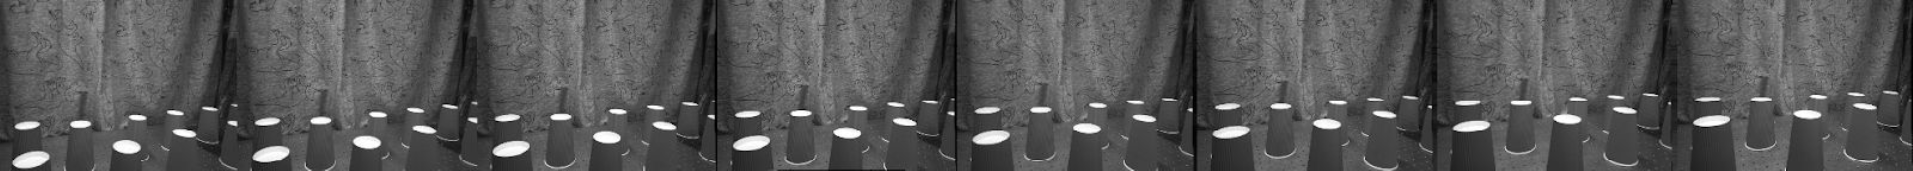
\includegraphics[width=6in]{images/epitile_3.png}
    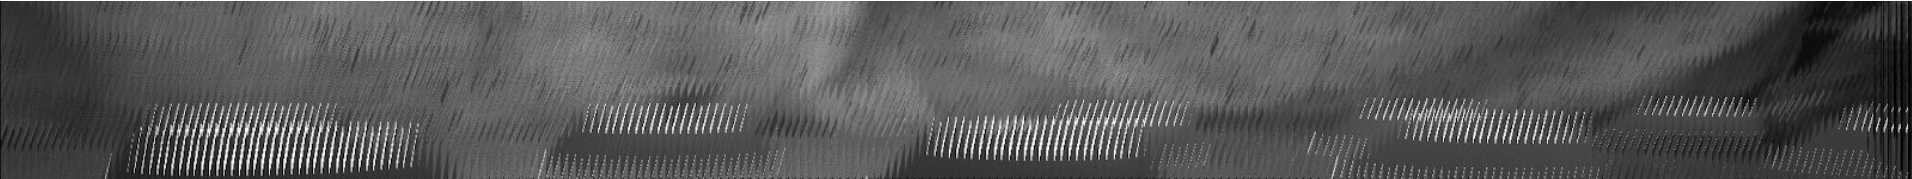
\includegraphics[width=6in]{images/epitile_2.png}
    \caption{Tiled \textit{U, V} slices (top): this is an intuitive way of slicing the light field, which tiles images from each sub-aperture side-by-side. Tiled \textit{T, V} slices (bottom): somewhat less intuitively, this method instead tiles the vertical epipolar-plane images side-by-side. We call these \textit{wide} EPIs. As shown, the overall dimensionality and shape of the light field is unchanged, we simply present the information in a different order, revealing different encodings of the captured scene. We can also tile the light field as \textit{S, U} slices, stacking them vertically, which we refer to as \textit{tall} EPIs.}
\end{figure}

\begin{figure}[H]
    \centering 
    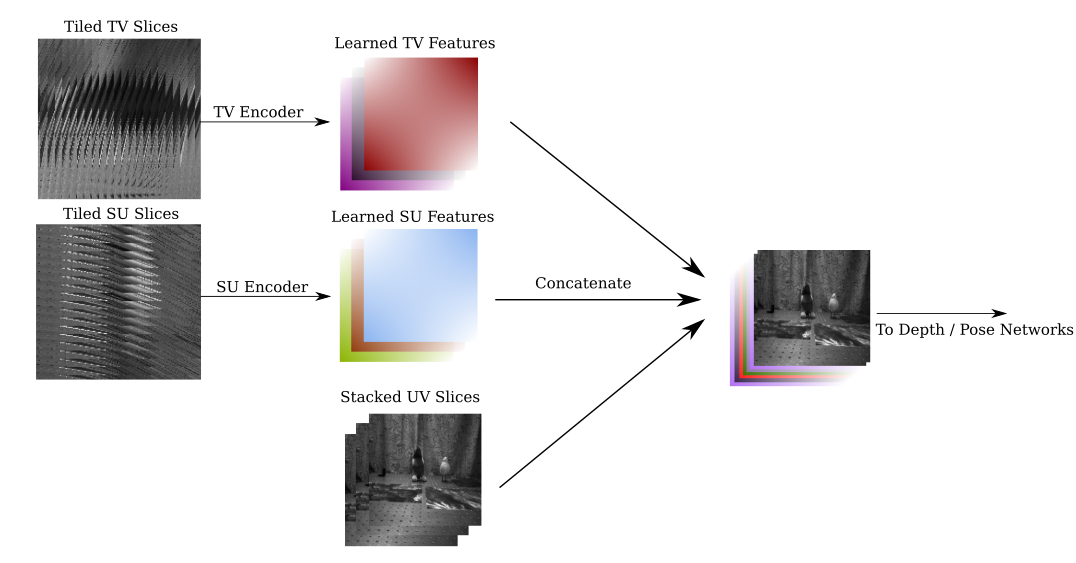
\includegraphics[width=6in]{images/encoderpipe.png}
    \caption{Our proposed encoder module which encodes the tiled EPIs, downsampling them to the shape expected by our depth and pose networks. Notably, features which have been learned in \textit{T, V} as well as \textit{S, U} are concatenated with the stacked \textit{U, V} slices (exactly as seen in our first input-method.) For brevity, we have only shown a small patch of the tall and wide EPIs, but the reader is reminded that these tilings are in fact very tall, and very wide.}
\end{figure}

\newpage

One challenge we face in ingesting this data, is that both previously described methods have input shapes $H \times W$. The tiled images from Figure 2.4 on the other hand have shape $H \times (W \times N)$ where $N$ is the number of sampled sub-apertures. In practice, these images are much wider than either of our previous input formats. We therefore suggest the use of an additional convolutional encoding module that down-samples the tiled EPIs to the shape expected by our depth and pose networks.

The encoding module consists of one convolutional layer followed by a ReLU activation layer. For the \textit{wide} EPIs we convolve with a kernel of size $N \times N$, and a horizontal stride of $N$. Zero-padding is applied to the top and bottom of the tiled EPI. The effect of this convolution is that the wide EPI is down-sampled with the same output size as a single \textit{U, V} slice. Similarly, we apply an $N \times N$ filter with a vertical stride of $N$ to the tall EPIs, also reducing their shape to that of a \textit{U, V} slice. The resulting feature-maps are combined with the \textit{U, V} slices, and provided to our depth and pose networks. Thus, our networks are able to learn features in three different feature-spaces. We hypothesise that with this ingestion strategy, our networks are able to learn an approximation for 4D signal processing functions, without the computational overhead of convolving in 4 dimensions, and without the requirement for a complete 2D grid of images.


\section{Complete Light Field Reconstruction}



In this section, we modify our pipeline to more-fully take advantage of the information in the light field. One important weakness of the pipeline we have described so far, is that there are no constraints on our networks to estimate scale with the same magnitude between video frames. Given three frames of video of the same scene, and stable camera motion, the depth network will happily estimate a room that is twice as large in the second pair of frames than the first, if of course the pose network also estimates a twice-as-large translation. This is the scale ambiguity that we have discussed in Chapter 2. With the modifications suggested in this section, we take advantage of the fact that we have multiple sub-apertures capturing the scene at the same time, using this knowledge to enforce scale consistency across video frames. 

The modification described here is straightforward, but it sacrifices some flexibility. The pipeline as we have described it so far requires only one vital piece of information to learn depth and visual odometry - the focal length of the camera being used (assuming all sub-apertures have very similar focal lengths). With this modification, we are required to at least know the arrangement of the sub-apertures in relation to one-another (although the absolute scale of their layout is not required). In our case, we know that our sub-apertures are arranged as a cross-hair. 

\begin{figure}[htbp]
    \centering 
    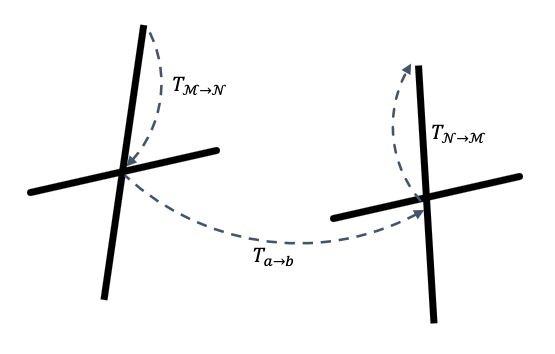
\includegraphics[width=3.5in]{images/relative_subapertures.png}
    \caption{Given knowledge of how one sub-aperture has moved through space, we can also compute how any other sub-aperture has moved by chaining the transforms in the order shown.}
\end{figure}

Instead of using photometric warp to reconstruct the image of a single sub-aperture, this modification adjusts the pipeline such that instead, we now reconstruct the entire light field. The camera array is a rigid body, meaning that as it rotates and translates through space, the sub-apertures also rotate and translate relative to each other, but in a very well defined way. Say we know the homogenous transform  $T_{a \rightarrow b}$ of sub-aperture $\mathcal{N}$ between two frames of video, we can compute the global transform of any other sub-aperture $\mathcal{M}$ by chaining together the homogenous transforms as shown in Figure 4.4.

To exploit this knowledge, we modify the depth prediction network to now output $N$ depth maps. Each depth map should be aligned with exactly one sub-aperture, so we can reconstruct its corresponding image. The pose network continues to estimate only the pose of the central sub-aperture, but the frame-to-frame pose for each pinhole is computed from the chained transform shown in Figure 4.4 (where $T_{a\rightarrow b}$ is the PoseNet output). For each sub-aperture we perform the same photometric warp with bilinear interpolation to synthesise $N$ viewpoints.

In addition to imposing a stronger supervision signal, this pipeline guarantees to a certain extent that our pose and depth modules predict depth at a consistent scale between video frames. We have enforced a photometric warp that requires prior knowledge of the shape of the camera, and with this information now making up a part of the photometric-warp pipeline, our neural networks are forced to learn to use this information to estimate depth and pose at the correct scale. To see why this is true, we should consider the effect on the loss function for an incorrectly estimated scale-factor. We may find that estimating a twice-as-large room for a twice-as-large translation works to photometrically warp the center-view well, but this will fail immensely for each of the other $N-1$ sub-apertures being warped. Thus, our networks are penalised harshly for incorrect scale estimates.

% \section{Experiments: Supervised Visual Odometry}

% A simple, yet revealing experiment is to train a model to perform visual odometry in a fully supervised setting. While unsupervised methods form a supervision signal by cleverly piecing together the available information, a fully supervised approach on the other hand theoretically produces the best possible results for any given system. Thus, there is a motivation to test the performance of the neural architectures described above. Not only does this experiment uncover what the pose network is capable of, but the experiment lays the groundwork for future unsupervised experiments. Individual modules such as the network itself, the data-loading module and even the weights of the trained network \footnote{While using pretrained weights to reduce training time is common practice, care is taken in this work to avoid using overlapping datasets when using pretrained weights. The dataset used to supervise the pre-trained weights should not contain the same scenes used to train the unsupervised model.} can be reused in future experiments. 

% \subsection{Monocular Visual Odometry}

% In the first iteration of this experiment, the KITTI dataset is used thanks to the size of the dataset and the availability of ground truth pose measurements. The input to the network is the pair of images in the sequence, and the loss function is computed from the ground truth 6-degree-of-freedom pose transform from one frame to the next. Evaluation is performed on sequences of the KITTI dataset that were withheld at training time, so as to gain an understanding of the models ability to generalise outside of the training data. 

% The network was trained for 18 hours, completing 70 passes over the input dataset. Stochastic gradient descent was used as the optimisation algorithm, using batch sizes of 8 images. The network was trained with pairs of image in both forwards and reverse order, meaning the network had to learn to predict both forwards and backwards motion. Input images were normalised with a mean pixel value at zero over the entire dataset, and divided by the standard deviation of the dataset. 


% \begin{figure}[htbp]
%     \centering
%     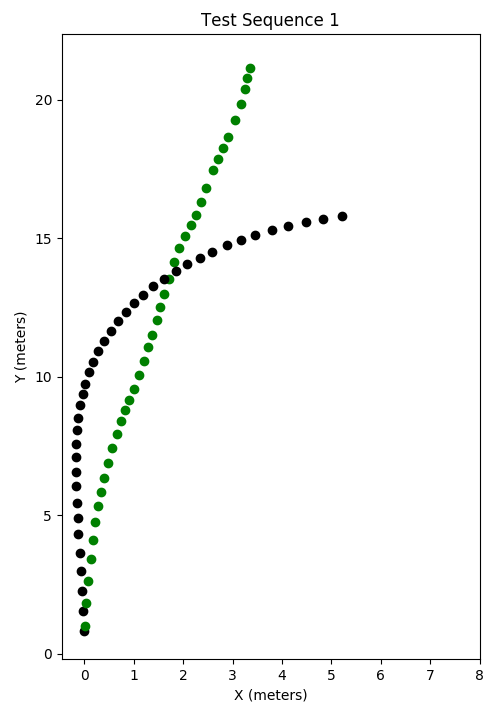
\includegraphics[height=2.4in]{images/vo_results/0034.png}
%     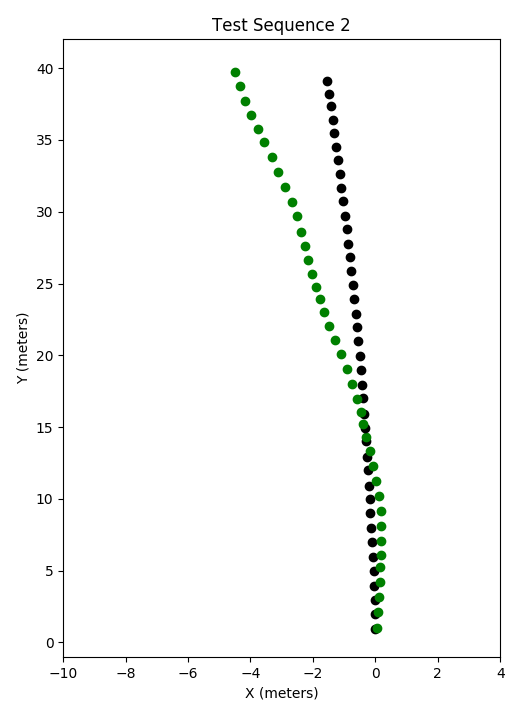
\includegraphics[height=2.4in]{images/vo_results/0018.png}
%     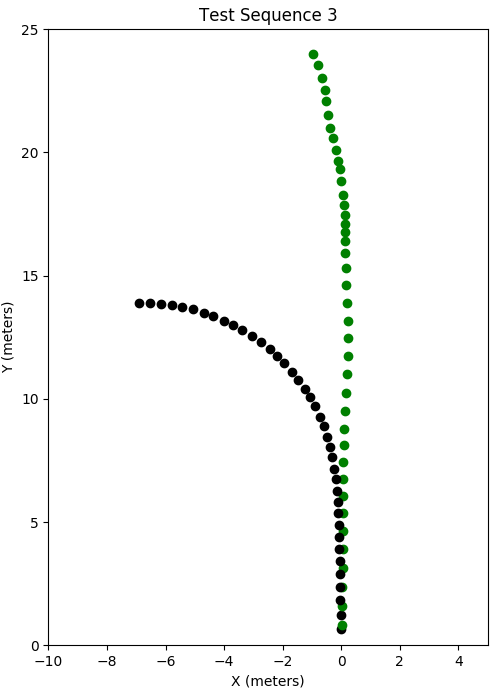
\includegraphics[height=2.4in]{images/vo_results/0027.png}
%     
\includegraphics[height=0.2in]{images/vo_results/legend.png}

%     \caption{Examples of trajectories generated from ground truth and estimated poses. These trajectories are generated over snippets of 40 frames from three test sequences which were withheld during training of the model. The cumulative nature of the error becomes more apparent the further the vehicle strays from the origin.}

%     \label{vo_results_kitti}
    
% \end{figure}

% \begin{table}[tbp]

%     \caption{Summary of Results for three test sequences}
%     \centering
%     \begin{tabular}{@{}llll@{}}
%         \toprule
%         Measure            & Sequence 1    & Sequence 2   & Sequence 3  \\ \midrule
%         Frames             & 40            & 40           & 40          \\
%         Path Length (m)    & 18.28         & 39.14        & 17.58       \\ \midrule
%         \multicolumn{4}{l}{Instantaneous Translational RMS Error (m)}   \\
%         X                  & 0.129         & 0.101        & 0.181       \\
%         Y                  & 0.013         & 0.034        & 0.018       \\
%         Z                  & 0.193         & 0.081        & 0.277       \\ \midrule
%         \multicolumn{4}{l}{Absolute Trajectory RMS Error (m)} \\
%         X                  &  0.81         & 1.39         & 2.70        \\
%         Y                  &  2.17         & 0.24         & 5.42        \\
%         Z                  &  0.12         & 0.37         & 0.25        \\ \bottomrule
    
%         \end{tabular}
%         \label{kitti_vo_results_tabular}
%     \end{table}



% Some examples of trajectories generated using raw-ground truth data and the predicted trajectories over 40 frame snippets of video are shown in Figure \ref{vo_results_kitti}. Because the trajectory of a vehicle driving along a road can be described almost entirely by its movements in a 2D plane, these trajectories are plotted as such, ignoring the minor up and down motions of the vehicle. While the error grows and becomes more evident at larger distances from the origin, the individual frame-to-frame error is qualitatively small. In observing these trajectories, we also note that while the network appears to have modeled forward and linear motion quite well, rotation seems to have been left behind. 

% Results from the experiment are reported in Table \ref{kitti_vo_results_tabular}. The table summarises the instantaneous translational errors from frame to frame as well as the absolute pose error of the cumulative trajectory. These errors are computed as the root-mean-square error of the distance between the predicted and ground truth poses for the 3 translation components. In this table, instantaneous translational errors are reported relative to the X-Y-Z coordinate frame of the camera (Z pointing out through the lens), while the absolute trajectory error is reported relative to the coordinate frames shown in Figure \ref{vo_results_kitti}.







% We observe in the tabulated results that the pose prediction consistently performs best in predicting translation in the $Z$ direction (up and down relative to the road). This is expected, as a vehicle driving on a flat road is likely to experience minimal up-and-down motion relative to the forwards-backwards and side-to-side components. The $Z$ translation of the cost function can thus be minimised easily by consistently predicting zero, or very close to zero for that component. Forwards and backwards instantaneous translations were predicted best in sequence two - a relatively straight stretch of road. This is indicative of the models difficulty when faced with tight corners as shown in sequences 1 and 3. 

% \subsection{Plenoptic Visual Odometry}
% A seemingly simple extension of the experiment described in the previous section is to perform the same procedure using light field imagery. With improved exposure to depth information, the model should see an improvement in performance, particularly in the awareness of scale. By providing multiple views, the model is able to implicitly learn the geometric features associated with the unchanging baseline between sub-apertures. This will aid in accurately predicting the magnitude of the rotations and translations in space. Such a model can learn to employ more robust features such as parallax and occlusion to estimate motion with improved scale awareness. After all, in the monocular case, the model must learn to infer scale from features of the scene (height above the ground or knowledge of the rough size of pedestrians could be features used by the model to make its predictions). 

% While the pose network is capable of ingesting light field imagery and a small dataset is ready for training with, experiments thus far have yielded numerically unstable training losses, even in the case of single sub-apertures - an effectively identical approach to the experiment described in the previous section. An investigation is currently underway into the reasons behind this instability. ß